\documentclass[border=2pt]{standalone}
% Build: pdflatex architecture_nolegend.tex  (from this folder) -> architecture_nolegend.pdf (variant without the responsibility boxes)
\usepackage{amsmath}
\usepackage{newtxtext,newtxmath} % Times, as in IEEEtran
\usepackage{xcolor}
\usepackage{tikz}
\usetikzlibrary{arrows.meta,fit,backgrounds}
\definecolor{archaccent}{RGB}{0,84,147}
\definecolor{archbroker}{RGB}{235,242,250}
\definecolor{archsite}{RGB}{244,244,244}
\definecolor{archcloud}{RGB}{253,243,230}
\definecolor{archcloudln}{RGB}{190,105,0}
\definecolor{archbusy}{RGB}{150,150,150}
\definecolor{archpred}{RGB}{233,245,233}
% \archpool{x}{y}{#busy of 5}{label}: a pool of identical on-premises nodes
\newcommand{\archpool}[4]{%
  \foreach \i in {0,...,4}{%
    \ifnum\i<#3\relax\def\archf{archbusy}\else\def\archf{white}\fi
    \draw[line width=0.4pt, fill=\archf] ({#1+\i*0.27},{#2}) rectangle ++(0.21,0.21);}
  \node[anchor=west, inner sep=1pt] at ({#1+1.36},{#2+0.105}) {#4};}
% \archvm{x}{y}{#running of 5}{label}: a cloud VM type; VMs exist only while used
\newcommand{\archvm}[4]{%
  \foreach \i in {0,...,4}{%
    \ifnum\i<#3\relax
      \draw[line width=0.4pt, draw=archcloudln, fill=archcloudln!45] ({#1+\i*0.27},{#2}) rectangle ++(0.21,0.21);
    \else
      \draw[line width=0.4pt, draw=archcloudln!70, dash pattern=on 1pt off 0.8pt] ({#1+\i*0.27},{#2}) rectangle ++(0.21,0.21);
    \fi}
  \node[anchor=west, inner sep=1pt] at ({#1+1.36},{#2+0.105}) {#4};}
% Author-facing notes; redefine as \newcommand{\revnote}[1]{} to hide them.
\providecommand{\revnote}[1]{{\color{red!70!black}\footnotesize[\textbf{TODO:} #1]}}

\begin{document}
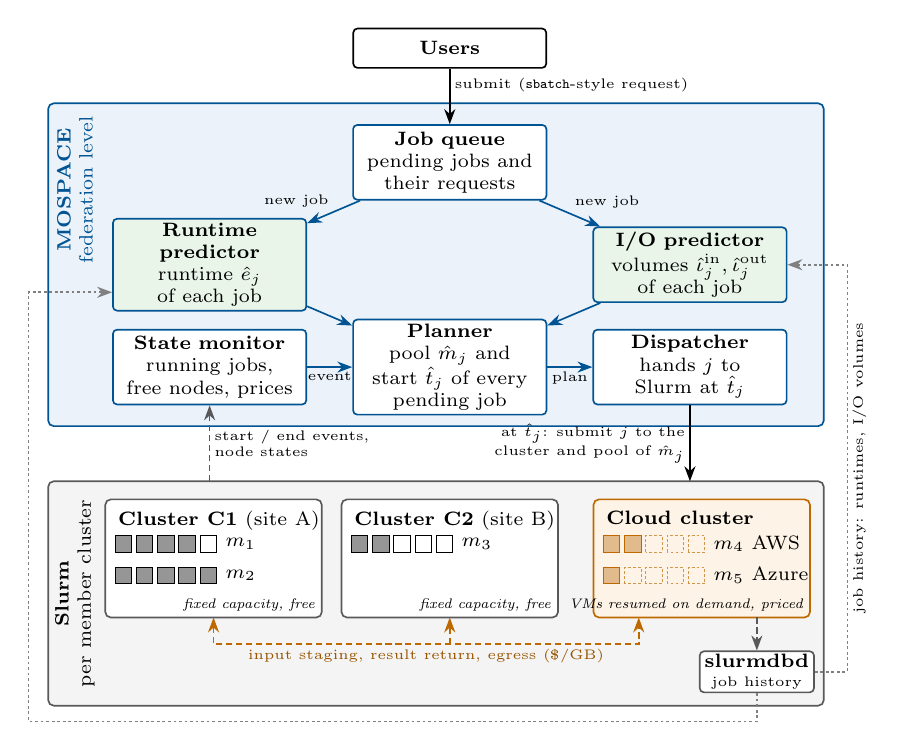
\begin{tikzpicture}[
  font=\scriptsize,
  >={Stealth[length=1.9mm,width=1.4mm]},
  comp/.style={draw=archaccent, fill=white, rounded corners=1.5pt, line width=0.6pt,
               minimum width=2.45cm, text width=2.35cm, minimum height=0.95cm,
               align=center, inner sep=1.5pt},
  pred/.style={comp, fill=archpred},
  flow/.style={->, line width=0.6pt, draw=archaccent},
  ctrl/.style={->, line width=0.7pt},
  ev/.style={->, line width=0.6pt, draw=black!65, dash pattern=on 2.2pt off 1.4pt},
  hist/.style={->, line width=0.6pt, draw=black!50, dash pattern=on 1pt off 1pt},
  data/.style={line width=0.6pt, draw=archcloudln, dash pattern=on 2.2pt off 1.4pt},
  grp/.style={rounded corners=2pt, line width=0.6pt, inner sep=0pt},
  clus/.style={grp, draw=black!65, fill=white, minimum width=2.75cm, minimum height=1.5cm},
  lbl/.style={font=\tiny, inner sep=1.5pt},
  layer/.style={rotate=90, align=center, font=\scriptsize},
  resp/.style={rounded corners=2pt, line width=0.6pt, text width=4.6cm, align=left,
               inner sep=3pt, anchor=north},
]
% ============================================ MOSPACE (federation level)
% submission -> queue -> both predictors in parallel -> planner -> dispatcher
\node[comp] (queue) at (4.4,0.55)   {\textbf{Job queue}\\ pending jobs and their requests};
\node[pred] (rtp)   at (1.35,-0.75) {\textbf{Runtime predictor}\\ runtime $\hat e_j$ of each job};
\node[pred] (iop)   at (7.45,-0.75) {\textbf{I/O predictor}\\ volumes $\hat\iota_j^{\mathrm{in}},\hat\iota_j^{\mathrm{out}}$ of each job};
\node[comp] (mon)   at (1.35,-2.05) {\textbf{State monitor}\\ running jobs, free nodes, prices};
\node[comp] (plan)  at (4.4,-2.05)  {\textbf{Planner}\\ pool $\hat m_j$ and start $\hat t_j$ of every pending job};
\node[comp] (disp)  at (7.45,-2.05) {\textbf{Dispatcher}\\ hands $j$ to Slurm at $\hat t_j$};

\draw[flow] (queue) -- node[above left, lbl] {new job} (rtp);
\draw[flow] (queue) -- node[above right, lbl] {new job} (iop);
\draw[flow] (rtp)   -- (plan);
\draw[flow] (iop)   -- (plan);
\draw[flow] (mon)   -- node[below, lbl] {event} (plan);
\draw[flow] (plan)  -- node[below, lbl] {plan} (disp);

\begin{scope}[on background layer]
  \node[grp, draw=archaccent, fill=archbroker, fit={(-0.7,1.3) (9.15,-2.8)}] (mos) {};
\end{scope}
\node[layer, text=archaccent] at (-0.36,0.2) {\textbf{MOSPACE}\\ federation level};

% submission
\node[draw, rounded corners=1.5pt, line width=0.6pt, minimum width=2.45cm,
      minimum height=0.5cm, font=\scriptsize\bfseries] (users) at (4.4,2.0) {Users};
\draw[ctrl] (users) -- node[right, lbl, pos=0.3] {submit (\texttt{sbatch}-style request)} (queue);

% ============================================ Slurm (cluster level)
\begin{scope}[yshift=-0.95cm]
\node[clus] (c1) at (1.4,-3.53) {};
\node[anchor=north west] at ([shift={(0.05,-0.03)}]c1.north west) {\textbf{Cluster C1} (site A)};
\archpool{0.15}{-3.45}{4}{$m_1$}
\archpool{0.15}{-3.85}{5}{$m_2$}
\node[lbl, anchor=south east, font=\tiny\itshape] at ([shift={(-0.04,0.03)}]c1.south east) {fixed capacity, free};

\node[clus] (c2) at (4.4,-3.53) {};
\node[anchor=north west] at ([shift={(0.05,-0.03)}]c2.north west) {\textbf{Cluster C2} (site B)};
\archpool{3.15}{-3.45}{2}{$m_3$}
\node[lbl, anchor=south east, font=\tiny\itshape] at ([shift={(-0.04,0.03)}]c2.south east) {fixed capacity, free};

\node[clus, draw=archcloudln, fill=archcloud] (cc) at (7.6,-3.53) {};
\node[anchor=north west] at ([shift={(0.05,-0.03)}]cc.north west) {\textbf{Cloud cluster}};
\archvm{6.35}{-3.45}{2}{$m_4$ AWS}
\archvm{6.35}{-3.85}{1}{$m_5$ Azure}
\node[lbl, anchor=south east, font=\tiny\itshape] at ([shift={(-0.04,0.03)}]cc.south east) {VMs resumed on demand, priced};

% data movement between sites
\draw[data, <->] (1.4,-4.28) -- (1.4,-4.62) -- (6.8,-4.62) -- (6.8,-4.28);
\draw[data, ->]  (4.4,-4.62) -- (4.4,-4.28);
\node[lbl, below, text=archcloudln!80!black] at (4.1,-4.62)
  {input staging, result return, egress (\$/GB)};

% accounting
\node[draw=black!65, fill=white, rounded corners=1.5pt, line width=0.6pt,
      minimum width=1.45cm, minimum height=0.5cm, align=center, inner sep=1pt]
  (dbd) at (8.3,-4.97) {\textbf{slurmdbd}\\[-1pt] {\tiny job history}};
\draw[ev] (8.3,-4.28) -- (dbd.north);

\begin{scope}[on background layer]
  \node[grp, draw=black!65, fill=archsite, fit={(-0.7,-2.55) (9.15,-5.4)}] (slm) {};
\end{scope}
\node[layer] at (-0.36,-3.975) {\textbf{Slurm}\\ per member cluster};
\end{scope}

% ============================================ interfaces between the layers
\draw[ctrl] (disp.south) -- node[left, lbl, align=right]
  {at $\hat t_j$: submit $j$ to the\\ cluster and pool of $\hat m_j$} (7.45,-3.5);
\draw[ev] (1.35,-3.5) -- node[right, lbl, align=left]
  {start / end events,\\ node states} (mon.south);
% job history (runtimes, I/O volumes) feeds both predictors
\draw[hist] (dbd.east) -- (9.45,-5.92) -- node[pos=0.5, right, lbl, rotate=90, anchor=north]
  {job history: runtimes, I/O volumes} (9.45,-0.75) -- (iop.east);
\draw[hist] (dbd.south) -- (8.3,-6.55) -- (-0.95,-6.55) -- (-0.95,-1.1) -- (rtp.west |- 0,-1.1);

\end{tikzpicture}
\end{document}
